\documentclass[tikz,border=5mm]{standalone}
\usepackage{amsmath}

\begin{document}

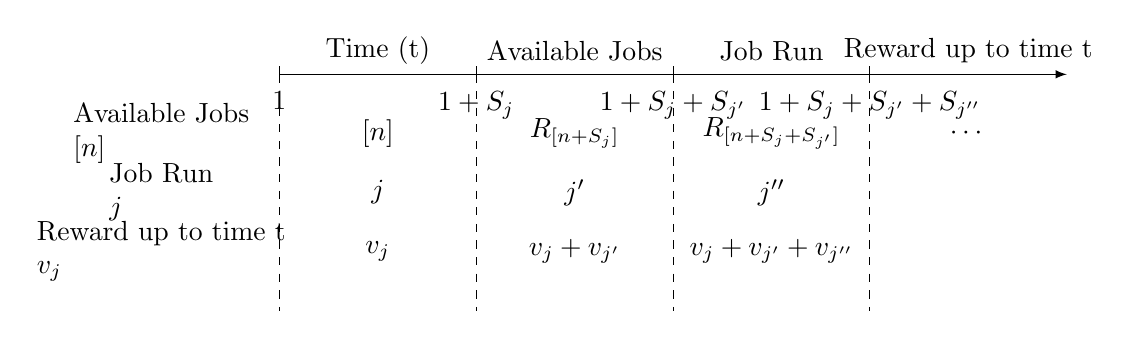
\begin{tikzpicture}[>=latex]

% Horizontal timeline
\draw[->] (0,0) -- (10,0);

% Time labels and vertical lines
\foreach \x/\label in {0/1, 2.5/1+S_j, 5/1+S_j+S_{j'}, 7.5/1+S_j+S_{j'}+S_{j''}} {
    \draw (\x,0.1) -- (\x,-0.1) node[below] {$\label$};
    \draw[dashed] (\x,0) -- (\x,-3);
}

% Horizontal labels
\node at (1.25,0.3) {Time (t)};
\node at (3.75,0.3) {Available Jobs};
\node at (6.25,0.3) {Job Run};
\node at (8.75,0.3) {Reward up to time t};

% Vertical labels
\node[align=left] at (-1.5,-0.75) {Available Jobs\\$[n]$};
\node[align=left] at (-1.5,-1.5) {Job Run\\$j$};
\node[align=left] at (-1.5,-2.25) {Reward up to time t\\$v_j$};

% Timeline labels
\node at (1.25,-0.75) {$[n]$};
\node at (3.75,-0.75) {$R_{[n+S_j]}$};
\node at (6.25,-0.75) {$R_{[n+S_j+S_{j'}]}$};
\node at (8.75,-0.75) {$\cdots$};

\node at (1.25,-1.5) {$j$};
\node at (3.75,-1.5) {$j'$};
\node at (6.25,-1.5) {$j''$};

\node at (1.25,-2.25) {$v_j$};
\node at (3.75,-2.25) {$v_j + v_{j'}$};
\node at (6.25,-2.25) {$v_j + v_{j'} + v_{j''}$};

\end{tikzpicture}

\end{document}